\documentclass{report}
\usepackage[utf8]{inputenc}
\usepackage{nicematrix}
\usepackage{xcolor}
\usepackage{graphicx}
\usepackage[frenchb]{babel}
\graphicspath{{images/}}
\usepackage[utf8]{inputenc}
\usepackage[T1]{fontenc}
\usepackage[french]{babel}
\usepackage{geometry}
\graphicspath{ {images/} }
\geometry{a4paper, total={170mm,257mm}, left=20mm, top=20mm,}
\begin{document}
% --------------------------------- PAGE DE GARDE ------------------------------
 
\author{Lucas ARIES, Paul DEVEAUX, Théo HORNBERGER, Terry TEMPESTINI}
\date{20 Octobre 2022}

\begin{center}
    \includegraphics[scale = 0.6]{telecom_nancy.png}
\end{center}

\begin{center}
    {\huge \textbf{Projet Jardi'Quest}} \\
    {\LARGE 
        PPII - Projet Pluridisciplinaire d'Informatique Intégrative \\
        Circuit-court et jardin partagé \\
        2022/2023
    }
    \vspace{1cm} \\
    {\LARGE \textbf{Responsables du module :}}
    \vskip 0.1cm
    {\Large 
    Oliver FESTOR \\ 
    Anne-Claire HEURTEL \\ 
    Gérald OSTER \\
    } 
    
    
    \vspace{1.3cm}
    {\LARGE \textbf{Équipe projet}} \\ 
    \vspace{0.2cm}
    \Large Lucas ARIES \\
    Paul DEVEAUX, \\ 
    Théo HORNBERGER \\
    Terry TEMPESTINI\\
    \vspace{3cm}
    \includegraphics[scale=0.4]{images/ul_logo.jpeg}  
\end{center}



\tableofcontents

% ---------------------------------- TABLE DES MATIERES -------------------------




% ---------------------------- ÉTAT DE L'ART -----------------------------------
\chapter{Projet PPII - Etat de l'art}

    Notre étude va se porter sur les cadres existants autour de notre projet, puis ensuite sera étudié différentes applications numériques mettant en oeuvre le sujet du projet. Pour faire une comparaison avec notre future application, un tableau comparatif a été créé. 
\section{Cadres existants :}

Tout d'abord, une aide gouvernementale a permis le financement de jardins partagés. En effet, le plan de relance économique “France Relance” a permis l’allocation de 17 Millions € au soutien de jardins partagés et collectifs. Les projets de jardins partagés doivent remplir plusieurs critères pour pouvoir accéder à cette allocation. Cette mesure concerne uniquement les zones urbaines et périurbaines et est seulement accessible par les collectivités,les bailleurs sociaux et les associations. L’aide est dédiée à des investissements matériels (comme des outils de jardins, des fournitures ou encore des équipements) et immatériels (prestations d'ingénierie ou études des sols). Par exemple, dans les Bouches du Rhône 500 000 euros ont été investi pour les jardins partagés et collectifs. Cette aide gouvernemental est le cadre existant autour de notre projet. Cela nous ammène donc maitenant sur les différentes application numériques déjà en place sur le marché des jardins partagés. Une étude comparatif a été réalisé avec notre futur projet. 


\section{Tableaux comparatif de l'analyse :}


\begin{tabular}{|p{3cm}|p{3cm}|p{3cm}|p{3cm}|p{3cm}|}
    \hline
    \textbf{Applications Critères} & \textbf{Adopte ma Tomate} & \textbf{Le potiron} & \textbf{Planter chez nous}
    \\ \hline
    \textbf{Possibilité de partager un jardin} & Partage sous forme d’annonces & Annonces & Annonces 
    \\ \hline
   \textbf{Possibilité de rejoindre un jardin} & Annonces & Annonces & Annonces  
    \\ \hline
   \textbf{Carte des jardins à proximité} & Carte de tous les jardins à proximité & Carte des annonces & Inexistant 
    \\ \hline
   \textbf{Conseils de jardinage} & Recommandation par saison et localisation & Blog avec articles & Sous formes d’articles 
    \\ \hline
    \textbf{Notifications} & Application smartphone et web & Application smartphone et web & Inexistant 
    \\ \hline
    \textbf{Utilisation professionnelle} & Compte professionnel disponible & Inexistant & Inexistant 
    \\ \hline
    \textbf{Échange de légumes} & Inexistant & Choix des légumes à échanger & Propositions sur le site 
    \\ \hline
    \textbf{Contact avec un jardinier} & Envoi de message & Coordonnées du jardinier & Inexistant 
    \\ \hline
   \textbf{Mise en place d’évènements} & Inexistant & Inexistant & Fête des légumes ou marchés 
    \\ \hline
    \textbf{Prêt de jardin} & Inexistant & Inexistant & Mise en relation avec le jardinier 
    \\ \hline
   \textbf{Forum} & Inexistant & Inexistant & Inexistant 
    \\ \hline
    \textbf{Format d'application ludique} & Inexistant & Inexistant & Inexistant 
    \\ \hline
\end{tabular}

\vspace{0.5cm} \\

\begin{tabular}{|p{3cm}|p{3cm}|p{3cm}|p{3cm}|p{3cm}|}
    \hline
    \textbf{Applications Critères} & \textbf{Click and Garden} & \textbf{Jardins de Noé} & \textbf{Prêter son jardin} 
    \\ \hline
    \textbf{Possibilité de partager un jardin} & Partage sous forme d’annonces & Annonces & Annonces sur le site
    \\ \hline
   \textbf{Possibilité de rejoindre un jardin} & Annonces & Annonces & Contact avec le propriétaire  
    \\ \hline
   \textbf{Carte des jardins à proximité} & Carte et filtres sur les régions & Inexistant & Inexistant
    \\ \hline
   \textbf{Conseils de jardinage} & Recherche guidée & Guide complet & Articles pédagogiques
    \\ \hline
    \textbf{Notifications} & Inexistant & Application web & Inexistant 
    \\ \hline
    \textbf{Utilisation professionnelle} & Inexistant & Rubrique "Jardins Professionnels" & Inexistant
    \\ \hline
    \textbf{Echange de légumes} & Inexistant & Inexistant & Fruits et légumes précisés
    \\ \hline
    \textbf{Contact avec un jardinier} & Inexistant & Inexistant & Inexistant  
    \\ \hline
    \textbf{Mise en place d’évènements} & Inexistant & Inexistant & Inexistant
    \\ \hline
    \textbf{Prêt de jardin} & Annonces par régions & Inexistant & Inexistant
    \\ \hline
    \textbf{Forum} & Inexistant & Forum Interactif & Inexistant 
    \\ \hline
    \textbf{Format d'application ludique} & Inexistant & Inexistant & Inexistant 
    \\ \hline
\end{tabular}

\section{Explication sur le choix des critères de comparaison :}
Les critères de comparaison que nous avons sélectionnés reposent tout particulièrement sur les attentes et les besoins des utilisateurs. Certains de ces critères seront indispensables à notre futur application, et il est donc primordial de connaître au mieux les différentes solutions proposées par les applications existantes. On peut citer, comme exemple, la possibilité de partager un jardin ou de rejoindre un jardin partagé. 
\newline
\\
D’autres critères répondent à un besoin de confort d'ergonomie pour l’utilisateur. On peut citer ici, les moyens de contacts des utilisateurs de la plateforme ou encore la disponibilité de conseils ou de forum. De plus, il est aussi particulièrement important de comparer la cible de ces applications. En effet, celles-ci sont généralement proposées à des particuliers, souvent des familles. Cependant, il faut aussi prendre en compte d'autres catégories de personnes qui pourraient être interessé par ce genre d'application. On peut citer que plusieurs de ces applications ont implantée une partie professionnelle. 
\newline
\\
Certains critères sont aussi utiles dans un aspect de différenciation par rapport aux autres plateformes. En effet, en comparant, des critères plus spécifiques et des idées originales auxquelles nous avons pu penser, cela pourrait nous permettre de nous différencier du marché actuel. Ici, ce sont les critères autour des possibilités d’échanges des légumes, la mise en place d'événements ou encore une application orienté autour d'un système ludique qui sont soulignés. 
\newline
\\
Cette liste de critères nous apporte donc les principales réponses des besoins auxquels nous devons répondre afin de satisfaire les futurs utilisateurs de notre application. Cependant, d’autres critères bien plus généraux sont aussi à prendre en compte. En effet, l’ergonomie générale du site ou la disponibilité de l’application sur tous les supports sont des critères qui ne sont pas spécifiques aux applications dédiées aux jardins partagés mais pour lesquelles nous devons aussi porter une attention particulière. \\
\newpage
% -------------------- FIN ETAT DE L'ART -----------------------------------

\chapter{Présentation du projet}
\section{Concept de l'application}

L'application est composé de deux types d'utilisateurs différents : les utilisateurs et les propriétaires. En fonction de leur statut, ils ont différentes actions possibles à leur disposition. 
\begin{itemize}
    \item Un utilisateur peut accéder à son jardin, au blog associé et aux différentes quêtes à réaliser. En revanche, s'il n'a pas de jardin, il aura la possibilité d'en rejoindre un au choix.
    \item Un propriétaire pourra déposer des quêtes à réaliser par les participants. Ces quêtes pourront être cycliques ou non.
\end{itemize}
Une économie est implantée dans chaque jardin, et elle lui est unique. Sa monnaie ne pourra pas être échangée avec celle d'un autre jardin. Elle est gagnable en réalisant des quêtes de jardinage. 
Le propriétaire pourra déposer les récoltes dans le marché, qui est également unique au jardin, et les participants du jardin pourront échanger la monnaie qu'ils ont accumulé contre les récoltes. 
\begin{center}
   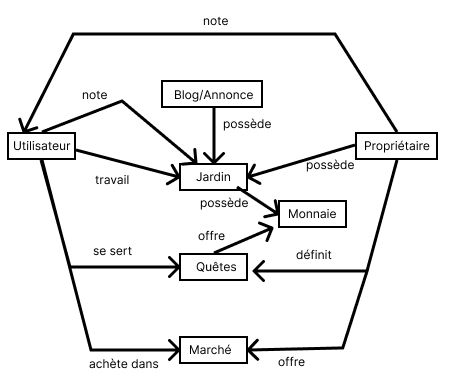
\includegraphics[scale=0.7]{images/Brainstorming-1.png}\\\\\\\\\\\
\end{center}

\section{Description du fonctionnement}

Un deuxième schéma de fonctionnement a été réalisé. Celui-ci représente les actions des différentes entités de l'application :

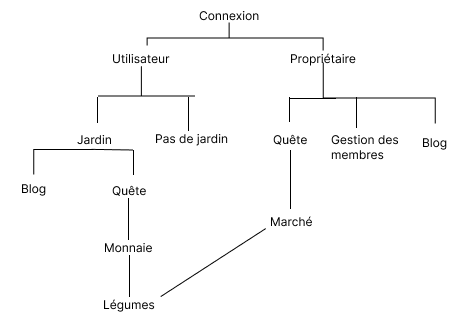
\includegraphics[scale = 0.7]{images/Brainstorming-2.png}\\

Les utilisateurs travaillent dans un jardin qu'un propriétaire a mis à disposition.
Les quêtes sont postées par le propriétaire et peuvent être cycliques ou non. Elles peuvent être réalisées par les jardiniers, ce qui leur rapporte un certaine quantité de monnaie virtuelle qu'ils peuvent échanger contre une quantité de légumes récoltés dans le jardin. C'est sur le marché que se passent ces échanges.
La partie blog est liée à toutes les personnes utilisant l'application et est présente pour améliorer la communications des utilisateurs.
\newpage


% -------------------- CHARTE PROJET -------------------------------------------
\chapter{Projet PPII - Charte}

\section{Auteurs}
\begin{tabular}{l|p{8cm}}
   \textbf{Nom / mél} & \textbf{Qualité / rôle}  \\
   \hline 
    DEVEAUX Paul & Membre du projet  \\
    paul.deveaux@telecomnancy.eu & \\ \hline
    HORNBERGER Théo & Membre du projet \\
    theo.hornberger@telecomnancy.eu & \\ \hline
    TEMPESTINI Terry & Membre du projet \\
    terry.tempestini@telecomnancy.eu & \\ \hline
    ARIES Lucas & Chef du projet \\
    lucas.aries@telecomnancy.eu & \\ \hline
\end{tabular}

\vspace{0.5cm}

\section{Historique des modifications et révisions de ce document}
\begin{tabular}{c|p{10cm}}
   \textbf{N° de version} & \textbf{Description et circonstances de la modification}  \\
   \hline 
    V.0.1 & Brouillon: préparation du documents
    \\\hline
    V 0.2 & Complétion du document
    \\ \hline
    V.1.0 & Relecture, reformulation des phrases et correction
\end{tabular}

\vspace{0.5cm}

\section{Validations / autorisations}
\begin{tabular}{c|p{4cm}}
   \textbf{N° de version} & \textbf{Nom / qualité} 
    \\ \hline  
    V 1.0 & ARIES Lucas 
\end{tabular}

\newpage


% ------------------------- Table des matières -------------------------------------

\section{Table des matières}

\section*{Résumé}
\subsection*{Cadrage}
\begin{itemize}
    \item La finalité du projet est la réalisation d'une application web qui a pour but de coordonner les différents participants d'un jardin partagé, et attirer un nouveau public à y participer.
    \item Le projet est réalisé en première année à Telecom Nancy dans le cadre du module PPII (Projet Pluridisciplinaire d'Informatique Intégrative) en groupe de 4 étudiants.
    \item Les objectifs de ce projet sont de :  
    \begin{itemize}
        \item Mettre en oeuvre la gestion de projet apprise pendant les cours
        \item Apprendre a travailler à plusieurs sur un même projet.
        \item De concevoir une application web possédant une partie base de données, web et algorithmique.
    \end{itemize}
\end{itemize}

\subsection*{Déroulement du projet}
\begin{itemize}
    \item L'organisation du projet est jalonnée par les différents rendus attendus par l'école. Il n'y a aucun temps sur l'emploi du temps consacré à celui-ci ni de budget, il est réalisé sur le temps libre des différents acteurs du projet.
    \item Les principaux évènements importants sont les réunions et les livrables imposés par le sujet tels que :
        \begin{itemize}
        \item Soutenance Gestion-Projet/État de l'art le 22/10/22.
        \item Rendu de projet le 06/01/23.
        \item Soutenance du projet le 14/01/23.
    \end{itemize}
    \item Les principaux risques sont les utilisateurs malveillants, et de sous-estimer le temps nécessaire à la réalisation des différentes tâches, et par conséquent de ne pas rendre les livrables dans les délais. Quant aux opportunités, celles-ci sont plutôt nombreuses notamment grâce à la situation économique actuelle.
\end{itemize}

\newpage

% ----------------------------------- Cadrage ----------------------------------



    \section{Cadrage}
   
    \subsection*{Contexte} 
    Les ressources naturelles deviennent de plus en plus rares et de plus en plus chères. La France, à l’instar de nombreux pays, est entrée dans un plan de sobriété économique. Cela se traduit par des mesures mises en place pour réduire notre consommation de ressources naturelles mais aussi notre consommation énergétique. 
    L’une des nombreuses idées pour contribuer à ce projet est d’inciter les consommateurs à se fournir leur alimentation via des circuits courts, c'est-à-dire des circuits impliquant le moins d’intermédiaires possibles, généralement aucun voir un seul. Cela permet alors de réduire la consommation énergétique liée au transport de marchandises, et donc leur coût. \\
    En parallèle, de nombreuses collectivités territoriales ont mis en place des jardins partagés, ce sont des jardins gérés et animés par des habitants d’un même quartier. En plus d’être une bonne alternative aux circuits courts d’un point de vue écologique et économique, cela permet de recréer un lien social, ce qui est le bienvenu après la crise de la Covid. \\
    
    L'objectif du projet est donc de créer un site web divertissant, ludique et simple d’utilisation qui améliorera la communication et la coordination des différents participants d’un jardin partagé. Il permettra aussi de répartir les récoltes de façon équitable. Voici les fonctions principales que l'application doit prendre en compte :
    \begin{itemize}
        \item Permettre aux utilisateurs de créer un jardin en renseignant les récoltes qui y sont effectuées, le nombre de places disponibles pour y participer, le lieu, ...
        \item Permettre aux utilisateurs de rejoindre un jardin existant.
        \item Créer une économie liée à un jardin en particulier. Chaque jardin possèdera sa propre monnaie, elle ne pourra pas être utilisée dans d’autres jardins.
        \item Permettre la création de quêtes. Leur objectif les besoins nécessaires à l’entretien des jardins. Les personnes les effectuant seront récompensées d’une certaine quantité de monnaie. Ces quêtes pourront être ponctuelles ou cycliques. Si elles sont cycliques, le délai avant qu'elles ne se répètent pourra être paramétré.
        \item Permettre la gestion d'un marché lié à un jardin. Les gérants du jardin pourront y proposer les récoltes du jardin contre de la monnaie. \item Permettre la communication entre différents participants du jardin.
        \item Permettre aux utilisateurs de déposer des avis sur d'autres utilisateurs 
        \item Intégrer un système de niveau qui récompense les utilisateurs actifs, via des quêtes qu'ils effectuent ou des avis qu'ils reçoivent.
    \end{itemize}

    De plus, l'application doit être réalisé en python, doit s'appuyer sur une base de données et doit être accessible via le web.\\
    
    La clientèle cible est donc tout d'abord les participants et gérants des jardins partagés, pour lesquels la communication doit être simplifiée. Cela se traduit par la liste des tâches restantes à accomplir dans le jardin et par le marché qui doit rendre le partage des récoltes plus équitables, mais également par un outil de discussion en ligne.
    Une autre clientèle, qui est novice des jardins, est visé. La ludification de l'application doit leur permettre d'appréhender le jardinage de manière plus amusante.
    
    
    \subsection*{Finalités}
    Ce projet a pour but de coordonner les différents participants d'un jardin partagé en aidant les gérants à mieux répartir les tâches nécessaires à l'entretien du jardin, ainsi qu'à mieux partager les récoltes. Il a également pour but d'inciter un nouveau public à s'intéresser aux jardins partagés, notamment les plus jeunes, grâce à de la ludification.\\
    
    La force du projet est qu'il est constitué d'une équipe qui a déjà acquis de l'expérience dans le développement d'application et qui a déjà vécu des conditions de travail en équipe similaires. Les tâches seront donc en théorie plus vite réalisées et mieux coordonnées qu'avec une équipe n'ayant jamais travaillé dans ces conditions. De plus, le projet ne comprend pas de budget, ce qui facilite la gestion de projet.\\
    Concernant les faiblesses, aucun des membres de l'équipe projet est spécialisé dans le front-end (mise en page de l'application). Les tâches relatives au front-end seront donc plus laborieuses. Les délais pour le projet sont également assez courts et l'équipe ne peut pas consacrer l'entièreté de son temps de travail sur le projet. Une très bonne organisation et répartition des tâches sera de mise. Pour finir, le marché est relativement méconnu de l'équipe. Les membres possèdent peu de connaissance dans le domaine du jardinage.\\
    
    
    
    \section{Livrables}
    Tout au long du projet, l'équipe projet devra rendre plusieurs livrables :
    \begin{itemize}
        \item Ensemble des fichiers sources des implémentations sur le dépot gitlab.
        \item Documentation sur le dépôt gitlab.
        \item Ensemble des documents produits relatifs à la gestion de projet.
        \item Rapport synthétique rédigé en LaTeX du travail sur l'état de l'art, décrivant l'application proposé et présentant en détails la gestion du projet. \textit{(20/10/2022)}
        \item Présentation en beamer ou Powerpoint de l'état de l'art réalisé, du concept de l'application visée et de son innovation. \textit{(22/10/2022)}
        \item Rapport rédigé en LaTeX synthétisant le travail et qui explique la conception et l'implémentation de l'application, une démonstration des tests et des performances, et l'explication de la gestion de projet. \textit{(06/01/2023)}
        \item Soutenance en beamer ou Powerpoint comportant des explications sur la conception et l'implémentation des différentes parties de l'application, une démonstration des fonctions, et des réponses aux questions. \textit{(14/01/2023)}
        
    \end{itemize}




% ------------------------------ Déroulement du projet ------------------------------
\section{Déroulement du projet}
\subsection*{Organisation / ressources, budget}
\begin{itemize}
    \item Le livret de mission du projet est le suivant : \\ 
    \textit{"Votre objectif est, en mettant en œuvre les principes de Gestion de Projet appris et
    ceux en cours d’acquisition dans le cours de gestion de projet et en mobilisant les acquis
    scientifiques et techniques du module CS54, de concevoir et d’implémenter une application
    innovante dédiée à l’optimisation des ressources dans les vergers et potagers du territoire}
    \item Rôles et responsabilités
    \begin{itemize}
        \item Équipe projet - Réalisation des différents livrables exigés.
        \item Équipe enseignante - Client du projet fixe les limites et demande les livrables.
    \end{itemize}
    \item Budget
    \begin{itemize}
        \item Financier 0€.
        \item Temps libre de 4 étudiants.
        \item Corps enseignant lié au module PPII.
    \end{itemize}
    
\end{itemize}
\subsection*{Jalons : échéancier / évènements importants }
Les différents évènements importants sont les réunions qui sont très régulières dues à la réalisation du projet avec les méthodes AGILES, mais aussi les différents livrables exigés qui rythme la vitesse de réalisation du projet.
\vspace{0.5cm} \\
La plupart des jalons importants sont répertoriés à l'aide de la todo-list suivante :

\begin{tabular}{|p{4cm}|c|c|c|p{3cm}|}
    \hline
    \textbf{Tâche} & \textbf{Pilote} & \textbf{Échéance} & \textbf{Durée} & \textbf{Commentaire}\\
    \hline
    Réfléchir au concept de l'application informatique & Équipe projet & 14/10/22 & 2 jours & Préparation de la réunion N°2\\
    \hline
    Réalisation de l'état de l'art & Terry, Théo & 17/10/22 & 3 jours & Documents LaTeX, analyse existant / concurrence\\
    \hline
    Gestion de projet & Paul, Lucas & 17/10/22 & 3 jours & SWOT, Todo List, charte du projet, cahier des charges \\
    \hline
    Regroupement travaux - Document Rendu 1 & Équipe projet & 20/10/22 & 3 jours & Documents a rendre à 18H \\
    \hline 
    Réalisation diaporama & Équipe projet & 21/10/22 & 2 jours & Réalisation et préparation de la présentation\\
    \hline
    Soutenance N°1 & Équipe projet & 22/10/22 & 0 jours & Samedi matin\\
    \hline 
    Compléter gestion de projet partie informatique & Équipe projet & & & Attente de plus d'informations\\
    \hline
    Rendu de projet & Équipe projet & 06/01/23 & & Gitlab\\
    \hline
    Réalisation diaporama N°2 & Équipe projet & 13/01/23 & 7 jours & Réalisation et préparation de la présentation\\
    \hline
    Soutenance N°2 & Équipe projet & 14/01/23 & & Fin du projet\\
    \hline
    Réflexion sur le projet et son organisation & Équipe projet & x & x & x\\
    \hline
    
\end{tabular}

\subsection*{Risques et opportunités}
Il y a différents risques et opportunités liés au déroulement du projet. \\ 
La principale opportunité pour le déroulement du projet est liée au corps enseignant qui représente un groupe d'experts qui est disponible pour répondre aux éventuelles questions, ou résoudre d'éventuels problèmes. \\ \\ 
De plus les jardins partagés deviennent de plus en plus courants notamment grâce à l'inflation des prix de l’alimentation, ce qui incite à produire et à manger local, mais aussi le plan de relance (France Relance) pour les jardins partagés. Le fait qu'aucun concurrent n'est implanté nationalement et ne domine le marché est également une grande opportunité. \\  \\ 
Quant aux risques possibles du projet, ceux-ci sont multiples :  \\ 
Que ce soit organisationnel, avec notamment des dates imposées pour les livrables et donc la possibilité de ne pas réussir à être dans les délais, mais aussi le fait qu'un nombre conséquent de projets concurrents risque de voir le jour en même temps que le notre. \\ 
De plus, le plus grand risque du projet est que celui-ci repose sur la bienveillance des utilisateurs et l'implication de ceux-ci dans leurs jardins.



% ------------------------------Conclusion -------------------------------

\chapter*{Conclusion}
La première étape a été de réaliser l'étude de l'existant pour apprendre le milieu du jardin partagé et de ce qui se fait. \\ 
Grâce à ceci nous avons pu concevoir une application originale qui apporte quelque chose aux utilisateurs de jardins partagés. Pour réaliser celui-ci dans des délais aussi court, nous avons réalisé de nombreuses réunions qui ont permis de répartir les différentes tâches tout en étant sûr que chaque membre de groupe ait la même vision du projet. \\ \\ 
Pour résumer celui-ci Jardi'Quest sera une application qui a pour objectif de rendre les jardins partagés ludique, comme un jeu et d'insister sur le mot "partagé" car actuellement ils sont le plus souvent découpé en parcelles. \\ 
Notre application a pour but de faire des jardins un travail d'équipe, qu'il soit entretenu par tous avec chaque membre apportant sa contribution à celui-ci a l'aide de quêtes.

% ---------------------------------- Annexes ---------------------------------
\newpage
\chapter*{Annexe}

\section*{Projet PPII - Compte rendu réunion N°1}
\begin{tabular}{|p{7cm}|p{6cm}|}
    \hline
    \textbf{Motif / Type de réunion :}
    & \textbf{Lieu :}
    \\
    Préparation du projet PPII
    & 
    Telecom Nancy
    \\ 
    Découverte des consignes &
    \\\hline
    \textbf{Présent(s)retard/excusés :}
    &
    \textbf{Date / Heure de début / Durée :}
    \\ 
    TEMPESTINI Terry &  13/10/22\\  
    DEVEAUX Paul & début 13h20\\
    HORNBERGER Théo & fin 14h40\\
    ARIES Lucas & 
    \\ \hline
\end{tabular}

\subsection*{Ordre du jour :}
\begin{itemize}
    \item{Repérer les différentes taches a réalisés}
    \item{Réfléchir a une idée d’application}
    \item{Organiser la répartition du travail}
\end{itemize}

\subsection*{Todo List :}
\begin{tabular}{|p{3.5cm}|c|c|p{4.5cm}|c|}
    \hline 
    Description & Responsable & Délai & Livrable & Validé par 
    \\ \hline
    Faire l’analyse de l’existant & x & 1 jour & x & x
    \\ \hline
    Réfléchir a une idée d’application web & x & 1 jour & x & x
    \\ \hline
\end{tabular}

\newpage

\section*{Projet PPII - Compte rendu réunion N°2}
\begin{tabular}{|p{7cm}|p{6cm}|}
    \hline
    \textbf{Motif / Type de réunion :}
    & \textbf{Lieu :}
    \\
    Finaliser l’idée, répartir tâches gestion de projet 
    & 
    Telecom Nancy
    \\ \hline
    \textbf{Présent(s)retard/excusés :}
    &
    \textbf{Date / Heure de début / Durée :}
    \\ 
    TEMPESTINI Terry &  14/10/22\\  
    DEVEAUX Paul & début 13h\\
    HORNBERGER Théo & fin 14h\\
    ARIES Lucas & 
    \\ \hline
\end{tabular}

\subsection*{Ordre du jour :}
\begin{itemize}
    \item{Définir clairement l’idée d’application}
    \item{Répartir les différentes tâches}
\end{itemize}

\subsection*{Todo List :}
\begin{tabular}{|p{3.5cm}|c|c|p{4.5cm}|c|}
    \hline 
    Description & Responsable & Délai & Livrable & Validé par 
    \\ \hline
    État de l’art & Terry, Théo & 3 jours &Document (Analyse de l’existant) & x
    \\ \hline
    Gestion de projet & Paul, Lucas & 3 jours & SWOT, charte de projet, todo-list & x
    \\ \hline
\end{tabular}


\newpage
\section*{Projet PPII - Compte rendu réunion N°3}
\begin{tabular}{|p{7cm}|p{6cm}|}
    \hline
    \textbf{Motif / Type de réunion :}
    & \textbf{Lieu :}
    \\
    Visualiser l'avancement du projet et redirigez le travail si nécessaire.
    & 
    Telecom Nancy
    \\ \hline
    \textbf{Présent(s)retard/excusés :}
    &
    \textbf{Date / Heure de début / Durée :}
    \\ 
    TEMPESTINI Terry &  17/10/22\\  
    DEVEAUX Paul & début 18h\\
    HORNBERGER Théo & fin 18h25\\
    ARIES Lucas & 
    \\ \hline
\end{tabular}

\subsection*{Ordre du jour :}
\begin{itemize}
    \item{Notifier l'avancement des tâches}
    \item{Organiser la prochaine réunion}
\end{itemize}

\subsection*{Todo List :}
\begin{tabular}{|p{3.5cm}|c|c|p{4.5cm}|c|}
    \hline 
    Description & Responsable & Délai & Livrable & Validé par 
    \\ \hline
    Terminer les différents documents & Équipe projet & 2 jours & Charte projet et état de l'art & Équipe projet
    \\ \hline
    Mettre en forme le rapport final & Équipe projet & 1 jours & Rapport final dû au jeudi & Équipe projet
    \\ \hline
\end{tabular}
\newpage
\section*{Projet PPII - Compte rendu réunion N°4}
\begin{tabular}{|p{7cm}|p{6cm}|}
    \hline
    \textbf{Motif / Type de réunion :}
    & \textbf{Lieu :}
    \\
    Préparation orale + Création Diaporama
    & 
    Telecom Nancy
    \\ \hline
    \textbf{Présent(s)retard/excusés :}
    &
    \textbf{Date / Heure de début / Durée :}
    \\ 
    TEMPESTINI Terry &  20/10/22\\  
    DEVEAUX Paul & début 13h40\\
    HORNBERGER Théo & fin 14h10h\\
    ARIES Lucas & 
    \\ \hline
\end{tabular}

\subsection*{Ordre du jour :}
\begin{itemize}
    \item{Vérifier le rapport final}
    \item{Réaliser le diaporama}
    \item{Préparer la soutenance}
\end{itemize}

\subsection*{Todo List :}
\begin{tabular}{|p{3.5cm}|c|c|p{4.5cm}|c|}
    \hline 
    Description & Responsable & Délai & Livrable & Validé par 
    \\ \hline
    Terminer le diaporama & x & 1 jour & x & x
    \\ \hline
    Préparer la soutenance & x & 1 jour & x & x
    \\ \hline
\end{tabular}

\newpage
\includegraphics[scale=0.75, angle=90]{gant.png}
\end{document}
